\documentclass[11pt]{article}
\usepackage{graphicx} % Required for inserting images
\usepackage{amssymb}
\usepackage{amsmath}
\usepackage[letterpaper, portrait, margin=1in]{geometry}
\usepackage{tabularx}
\usepackage{pgfplots}
\usepackage{tikz}
\usepackage{subfig}
\pgfplotsset{compat=1.18}

\usepackage{natbib}
\bibliographystyle{unsrtnat}
%\usepackage[breaklinks,hidelinks]{hyperref}
\usepackage[hyphens]{url}


\usepackage{fancyhdr}
\usepackage{lipsum}% just to generate some text
\usepackage{lastpage}


\setlength{\parskip}{.5\baselineskip}
\setlength\parindent{0pt}

%\fancypagestyle{fancy}
%{
%    \renewcommand{\headrulewidth}{0.4pt}
%
 %   \lhead{CHRIS RAYMOND-BERTRAND}
 %   \rhead{Page \thepage  \;of \pageref{LastPage}}
    
 %   \fancyfoot[C]{} 
%}

%\pagestyle{fancy}

\definecolor{accent}{RGB}{0,100,180}
\definecolor{loss}{RGB}{200,50,50}

\newcommand{\uu}{\mathbf u}
\newcommand{\vv}{\mathbf v}
\newcommand{\xx}{\mathbf x}
\newcommand{\yy}{\mathbf y}
\newcommand{\zz}{\mathbf z}
\newcommand{\bb}{\mathbf b}
\newcommand{\ah}{\hat a}
\renewcommand\aa{\mathbf a}
\newcommand{\lra}{\Leftrightarrow}
\newcommand{\tr}{^\text{T}}
\newcommand{\sep}{\;|\;}
\newcommand{\gauss}{\sim \mathcal{N}}

\DeclareMathOperator{\mf}{\mathbf }
\newcommand{\R}{\mathbb{R}}
\newcommand{\Z}{\mathbb{Z}}
\newcommand{\E}{\mathbb{E}}
\DeclareMathOperator{\pf}{\;\forall}
\DeclareMathOperator{\tif}{\text{ if }}

\newcommand{\bn}{\bigskip\noindent}
\newcommand{\bs}{\bigskip}
\newcommand{\nin}{\noindent}
\newcommand{\te}{\text}
\newcommand{\mb}{\mathbf}
\newcommand{\Var}{\text{Var}}

\newcommand{\inv}{^{-1}}
\newcommand{\pid}{\Phi^{-1}(\Delta)}

\newcommand{\lp}{\left(}
\newcommand{\rp}{\right)}
\newcommand{\lb}{\left\{}
\newcommand{\rb}{\right\}}
\newcommand{\lbk}{\left[}
\newcommand{\rbk}{\right]}

\renewcommand{\a}{\alpha}
\newcommand{\D}{\Delta}
\renewcommand{\P}{\Phi}
\newcommand{\p}{\phi}
\newcommand{\Pinv}{\Phi^{-1}}

\renewcommand\thesubsection{\alph{subsection}}

\newcommand{\norm}[1]{\left\lVert#1\right\rVert}
\title{DRO Stochastic Markowitz portfolio with SOCP}
\author{Chris Raymond-Bertrand}
\date{June 2025}

\title{\vspace{-.5in}Portfolio Optimization with Censored Return Distributions}
\author{Chris Raymond-Bertrand \& Cinar Ari}
\date{\today}

\begin{document}

\maketitle


%\section{Lit review}
%
%Robustifying Conditional Portfolio Decisions via Optimal Transport
%\begin{itemize}
%    \item Similar idea, but way different methods
%    \item They use joint distributions of returns and covariates, and the robustness comes from ambiguity in the joint distribution of X and Y
%    \item Solved using Optimal Transport model
%\end{itemize}


\section{Introduction}
A major problem in finance is portfolio optimization: Given a set of $n$ risky assets, how should the wealth be distributed among these asset for the best return to risk ratio? One approach was studied in the seminal paper \cite{markowitz1952}. One of the stated conclusion is that one should try to find the minimum variance portfolio for a given level of expected return by utilizing negatively or non-correlated assets. The formulation yields a convex quadratic optimization problem which is still widely used today.

This project aims to introduce put options as additional financial instruments that the investor can utilize in the Markowitz model. We investigate if one can get a better portfolio by simultaneously optimizing both the portfolio weights as well as put option levels compared to the standard Markowitz model. Our model introduces an additional decision variable $\Delta_i$, which represents the probability that the insurance bought is actually used (or, using the finance terminology, in the money). Once the investor decides on $\Delta_i$, the strike price and the cost of the put (priced using the Black-Scholes formula) is automatically determined. 

A big challenge in this model is to determine the moments of the return distribution. The return of each protected asset follows a censored normal distribution rather than a normal distribution. We derive closed form expressions for the moments of the censored normal distribution. The second challenge is that, in contrast to the original convex quadratic Markowitz formulation, the distribution, and hence the moments of returns depend on the decision variable $\Delta_i$. This results in a highly nonconvex optimization problem. We use approximations when necessary to keep the problem tractable. In particular, we replace the normal CDF, PDF, and inverse CDF with low-order polynomial approximations. 

We test our model using the approximations in Gurobi and show that inclusion of protective put options can reduce the variance of the portfolio with minimal changes in returns.


\section{Literature review}

Portfolio optimization theory begins with \cite{markowitz1952}. Markowitz formulated the problem as a convex quadratic optimization problem, where the objective is to minimize the variance for a given level of expected return. This set of minimum variances for different expected returns form an efficient frontier. \cite{sharpe1964} extended this model into the Capital Asset Pricing Model (CAPM). CAPM additionally has a risk-free asset and utilizes the Sharpe ratio to measure the performance. In our work, we also consider both variance minimization and also the Sharpe ratio.

Introducing put options to portfolio optimization problems is not a new idea. Although not exhaustive, we give an overview of certain ideas in the literature. \cite{leland1980} showed that put options can guarantee a minimum portfolio value and demonstrated options can be a valuable asset for some investors. \cite{ahn1999} and \cite{haugh2001} showed that with options, the introduced nonlinearity removes the convexity property of the efficient frontier and the Markowitz model. The paper by \cite{alexander2006} proposed that one can use CVaR instead of the variance to test the effectiveness of options. In our work, we do a joint optimization of both the option levels as well as portfolio weights and to the best of our knowledge, such work is new to the literature.

A big limitation of mean-variance optimization is the sensitivity to estimation errors. There is a big body of work in the literature to reduce the impact of estimation errors, such as covariance shrinkage \cite{ledoit2004}, robust formulations \cite{goldfarb2003}, and Bayesian priors \cite{black1992}.

\section{Put options}\label{sec:putoptions}

A (European) put option with strike price $K$ is a contract that gives the right to the holder to sell the underlying asset at the strike price $K$ at the expiration date. The payoff of the put option at the expiration date is $\max(K - S', 0)$ where $S'$ is the price of the asset at the expiration date.

In our work, we allow the investor to buy put options for insurance purposes. This means, the investor must hold the asset in order to be able to purchase the put. This way, the price floor of the asset is set to at least $K$. Clearly, such a protection cannot be free. The investor must pay a price $P$ at the time of purchase of the option. The optimization problem here is to balance the tradeoff between $P$ and the benefit of the put option. In Figure \ref{fig:protective_put}, payoff of a protective put option (i.e., while holding the asset as well as the stock) can be seen.

\begin{figure}[ht]
\centering
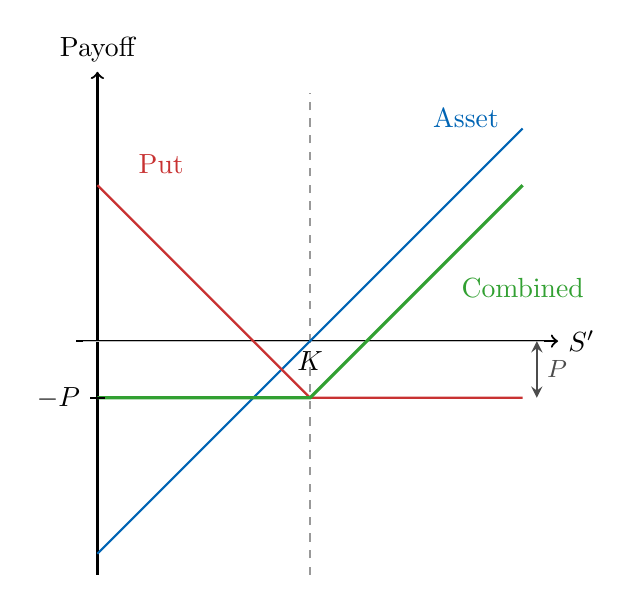
\begin{tikzpicture}[scale=0.9, thick]
  \definecolor{accent}{RGB}{0,100,180}
  \definecolor{loss}{RGB}{200,50,50}
  \definecolor{gain}{RGB}{50,160,50}
  \def\P{0.8}
  % Axes
  \draw[->] (-0.3,0) -- (6.5,0) node[right] {$S'$};
  \draw[->] (0,-3.3) -- (0,3.8) node[above] {Payoff};
  % Strike price marker
  \draw[dashed, black!40] (3,-3.3) -- (3,3.5);
  \node[below] at (3,0) {$K$};
  % Zero line
  \draw[black!25, thin] (-0.2,0) -- (6.3,0);
  % Asset payoff: S' - k
  \draw[accent, thick] (0,-3) -- (6,3);
  \node[accent] at (5.2,3.15) {Asset};
  % Put payoff net of premium: max(k - S', 0) - P
  \draw[loss, thick] (0,{3-\P}) -- (3,{-\P}) -- (6,{-\P});
  \node[loss] at (0.9,2.5) {Put};
  % Combined payoff: max(S', k) - k - P
  \draw[gain, very thick] (0,{-\P}) -- (3,{-\P}) -- (6,{3-\P});
  \node[gain] at (6,0.75) {Combined};
  % Mark -P on y-axis
  \draw[thick] (-0.1,{-\P}) -- (0.1,{-\P});
  \node[left] at (-0.1,{-\P}) {$-P$};
  % Annotation: brace showing the cost P shifts the floor down
  \draw[<->, >=stealth, black!70] (6.2,0) -- node[right] {\small $P$} (6.2,{-\P});
\end{tikzpicture}
\caption{Protective put payoff diagram}
\label{fig:protective_put}
\end{figure}

The cost of a put option is determined by the Black-Scholes formula \citep{black1973}:
\begin{equation}\label{eq:black_scholes}
    P = K \, e^{-rT} \, \Phi(-d_{2}) - S \, \Phi(-d_{1}),
\end{equation}
where $S$ is the current price of the asset, $r$ is the risk-free rate (RFR), $T$ is the time to expiration, and
\begin{equation}\label{eq:black_scholes_ds}
    d_{1} = \frac{\ln(S/K) + T(r + \sigma^2 / 2)}{\sigma \sqrt{T}}, \qquad
    d_{2} = d_{1} - \sigma \sqrt{T}.
\end{equation}

\subsection{Characterization of the combined return distribution}

%Let $X\sim \mathcal{N}(\mu, \sigma^2)$ be the returns of a particular stock.
Let $X\sim \mathcal{N}(0, 1)$ be the returns of a particular stock --- we will focus on non-normalized distributions in Sec.~\ref{sec:scale_shift}. Let $\phi$ be the normal PDF, and $\Phi$ be the normal CDF. Define $r(x, \alpha): \R \times \R \to \R$ as the return distribution for a stock with normally distributed returns with capped downside/breakpoint $\alpha$. 
\begin{equation} \label{eq:returns}
    r(x, \alpha) = 
\begin{cases}
    x \quad &\te{if } x > \alpha \\
    \alpha & \te{if }x \leq  \alpha \\
\end{cases}
\end{equation}
This gives us the resultant PDF $f(x, \alpha): \R\times \R \to \R_+$:
\begin{equation} \label{eq:pdf}
    f(x, \alpha) = 
\begin{cases}
    \phi\left( x\right) \quad &\te{if } x> \alpha \\
    \delta(\alpha) \cdot \Phi(\alpha) & \te{if }x = \alpha \\
    0 &\te{if } x< \alpha
\end{cases}
\end{equation}
, where $\delta$ is the Dirac function, defined as $\delta(a) = \begin{cases}
    +\infty & x=a\\ 0 &\te{otherwise}
\end{cases}$, and $\int_{-\infty}^{+\infty} \delta(x)dx= 1$. Thus, on $(\alpha, +\infty)$, we recover the stock's original distribution, while the $ \delta(\alpha) \cdot \Phi(\alpha)$ term concentrates its left-tail at the breakpoint. This type of distribution, often called a \textit{censored} or \textit{Tobit} distribution, is particularly useful in statistics, where observations might lie outside a predefined observable range, and thus concentrate the tails of the underlying distribution at the edges of said range.  

\subsubsection{First and second moments}

\cite{recursive_moments} has derived recursive formulae for the moments of the truncated normal term. We then use the law of total expectation to find the moments of $f(x, \alpha)$. 
\begin{equation}\label{eq:first_moment}
\begin{aligned}
\E[f(x, \alpha)] &= \E[f(x, \alpha) | X \leq \alpha]\cdot P (X \leq \alpha) + \E[f(x, \alpha) | X > \alpha]\cdot P (X > \alpha) \\
&=\alpha \Phi(\alpha) + \left( \frac{\phi(\alpha)}{1-\Phi(\alpha)}\right)\cdot(1-\Phi(\alpha)) = \alpha \Phi(\alpha) + \phi(\alpha)
\end{aligned}
\end{equation}
For the second moment, we get
\begin{equation}\label{eq:second_moment}
    \begin{aligned}
\E[f(x, \alpha)^2] &= \E[f(x, \alpha)^2 | X \leq \alpha]\cdot P (X \leq \alpha) + \E[f(x, \alpha)^2 | X > \alpha]\cdot P (X > \alpha) \\
&=\alpha^2 \Phi(\alpha) + \left( 1+\frac{\alpha\phi(\alpha)}{1-\Phi(\alpha)}\right)\cdot(1-\Phi(\alpha)) \\
&= \alpha^2 \Phi(\alpha) + 1-\Phi(\alpha) +\alpha\phi(\alpha)=\Phi(\alpha)(\alpha^2-1)+\alpha\phi(\alpha)+1
\end{aligned}
\end{equation}

\subsubsection{Expectation and variance}
Let $\mu^\alpha$ represent the true expectation of the distribution. The best estimator for $\mu^\alpha$ is $\E[f(x, \alpha)]$. So
\begin{equation}\label{eq:censored_mu}
   \mu^\alpha = \E[f(x, \alpha)] = \a\Phi(\a)+\phi(\a) 
\end{equation}
Using the identity $\sigma^2 = \E[X^2] -\E[X]^2$, combining Eqs.~\ref{eq:first_moment},~\ref{eq:second_moment}, $\left(\sigma^\alpha \right)^2$ can be computed as
\begin{equation}\label{eq:censored_var}
\begin{aligned}
\left(\sigma^\alpha \right)^2 &= \E[f(x, \alpha)^2] -\E[f(x, \alpha)]^2 \\
&= \Phi(\alpha)(\alpha^2-1)+\alpha\phi(\alpha)+1 - \lp \alpha \Phi(\alpha) + \phi(\alpha) \rp^2 \\
&= \Phi(\alpha)(\alpha^2-1)+\alpha\phi(\alpha)+1 - \lp\alpha^2 \Phi(\alpha)^2 + 2\alpha \Phi(\alpha)\phi(\alpha) + \phi(\alpha)^2\rp \\
&=  \Phi(\a)\a^2(1-\Phi(\a)) + \phi(\a)(\a-2\a \Phi(\a)-\phi(\a))-\Phi(\a)+1
\end{aligned}
\end{equation}

\subsection{Non-normalized censored return distributions}\label{sec:scale_shift}

Assume  $Y\sim \mathcal{N}(\mu, \sigma^2)$. By the properties of the normal distribution, $Y \sim \sigma X+\mu$. Being a linear transformation, we obtain the following results for this new distribution, using standard expectation and variance identities:
\[
\begin{aligned}
    \E[Y] &= \mu+\sigma E[f(x)] = \mu + \sigma\mu^\alpha = \mu+\sigma\lbk \alpha\Phi(\a) +\phi(\a)  \rbk \\
    \Var[Y] &=  \sigma^2\Var[f(x)] = \sigma^2 \left(\sigma^\alpha \right)^2 = \sigma^2[\Phi(\a)\a^2(1-\Phi(\a)) + \phi(\a)(\a-2\a \Phi(\a)-\phi(\a))-\Phi(\a)+1]
\end{aligned}
\]
Observing a distribution whose left-tail has been eliminated, one would expect that the resultant censored distribution will always have greater expectation than the underlying asset. In particular, this excess return can characterized by the factor of $\sigma\mu^\alpha = \sigma\lbk \alpha\Phi(\a) +\phi(\a)  \rbk \geq 0$, which is strictly increasing in $\a$. Looking at the limits, $\lim_{ \a \to -\infty}\sigma\mu^\alpha = 0$,  meaning that the expectation of the censored distribution approaches the expectation of the underlying distribution for $\alpha \ll \mu$. As $\alpha$ increases, $\Phi(\a) \to $ and $\phi(\a) \to 0$, so the expectation approaches $\sigma\alpha$ for $\a \gg \mu$.

Similarly interesting characteristics can be observed for the variance. which will also always be lower than the original variance. $\sigma^\alpha$ is strictly decreasing in $\a$, with $\sigma^\alpha \to \sigma$ for $\alpha \ll \mu$, and $\sigma^\alpha \to 0$ for $\a \gg \mu$.

Thus, as expected, when $\a \to +\infty$, we recover the original uncensored distribution, and with large $\a$, we approach a guaranteed return of $\a$.

\subsection{Covariance}

Unfortunately, formulae for covariance of two censored distributions is, as far as we know, unable to be found in the literature, due to the highly complex interactions between the two distributions. Given the correlation coefficient $\rho_{ij}$ between assets $i, j$, with breakpoints $\a_i, \a_j$ we approximate the covariance of the two distributions as
\begin{equation}\label{eq:covar}
\begin{aligned}
\text{Covar}[X_i, X_j] &\approx \sigma_i\sigma_j\rho_{ij}\cdot P(X_i>\alpha_i)\cdot P(X_j>\a_j) \\
    &=\sigma_i\sigma_j\rho_{ij}[1-\P(\a_i)][1-\P(\a_j)]
\end{aligned}
\end{equation}
The rational behind this approximation is 
\begin{itemize}
    \item Limit preservation: as $\a_i, \a_j \to -\infty$, we recover the original covariance, and as $\a_i, \a_j \to +\infty $, the covariance goes to 0. 
    \item Interpretability: the covariance shrinks by the proportion of the distribution that has been truncated.
    \item Preservation of positive definiteness: further discused below
\end{itemize}
Thus, our covariance matrix $\Sigma^\a$, can be written as 
\[
\begin{aligned}
    \Sigma^\a_{ii} &= (\sigma_i^\a)^2 &&\forall i \\
    \Sigma^\a_{ij} &= \sigma_i\sigma_j\rho_{ij}[1-\P(\a_i)][1-\P(\a_j)] &&\forall i, j: i\neq j
\end{aligned}
\]
Which can be equivalently written as 
\[
\Sigma^\a = \Sigma\circ \mathbf{p}\mathbf{p}^T +D
\]
, where $\Sigma$ is the original distribution's covariance matrix, $\circ$ is the Schur or element-wise product of two matrices, $\mathbf{p}^T = \begin{bmatrix}
    1-\Phi(\a_1)  &
    \hdots &
    1-\Phi(\a_n)
\end{bmatrix}$, and $D=\te{diag}\lp \lp\sigma_i\sigma_{i}^\alpha \rp ^2 \rp - \te{diag}\lp\sigma_i^2[1-\P(\a_i)]^2]\rp$, i.e. a diagonal matrix representing the difference between an asset's true censored variance, and the censored variance returned by the approximation.

Let us show that this matrix remains positive-definite (PD). First, the Schur product of two positive semi-definite (PSD) matrices is also PSD. $\Sigma$ is PSD by construction, and $\mathbf{p}\mathbf{p}^T$ is a rank-1 matrix whose only eigenvalue is $\norm{\mathbf{p}}_2^2 \geq 0$, so $\mathbf{p}\mathbf{p}^T \succeq 0\implies \Sigma \circ \mathbf{p}\mathbf{p}^T \succeq 0$. As for $D$, the difference of two diagonal matrices is diagonal, and in this case, each $D_{ii} >0 \implies D\succ 0$. The sum of a PSD matrix with a PD matrix is PD, so $\Sigma^\a \succ 0$.

This guarantees that the resultant covariance matrix $\Sigma^\alpha \succ0\implies w^T\Sigma^\a w > 0 \;\forall w : \|w\|_1=1$, meaning $\sqrt{w^T\Sigma w}$ is well-defined.



\section{Optimization model}

In classical Markowitz optimization, a decision-maker seeks to find an optimal allocation of resources into a given set of assets. Each asset has a given expected return $\mu_i$, variance $\sigma_i$, and assets $i, j$ are correlated with coefficient $\rho_ij$. One form of the problem (Eq.~\ref{eq:reg_markowitz}) seeks to maximize the expected portfolio return, while keeping the portfolio variance below a specific threshold. Another version is to minimize the variance, given a minimum expected return, but both versions are equivalent.

Another measure of portfolio performance is the Sharpe ratio \citep{sharpe1964}, which corresponds to the excess returns above a risk-free baseline $r_f$, divided by the variance of the returns (Eq.~\ref{eq:naive_sharpe}).

%\begin{aligned}
 %   &\max \sum_{i=1}^n \mu_i w_i\\
  %  \text{s.t.}\quad& \sqrt{w^T\Sigma w} \leq \sigma_{\max}\\
   % & \sum_{i=1}^n w_i = 1\\
    %&\qquad w_i \geq 0
%\end{aligned}
%\qquad\Longleftrightarrow\qquad
\begin{subequations}
\begin{minipage}{0.45\textwidth}
    \vspace{-.5cm}
    \begin{equation}\label{eq:reg_markowitz}
        \max_{w \in \mathcal{W}} \mu^T w
        \quad \text{s.t.} \quad \left\|\Sigma^{\frac{1}{2}}w\right\|_2 \leq \sigma_{\max}
    \end{equation}
\end{minipage}
\hfill
\begin{minipage}{0.45\textwidth}
    \begin{equation}\label{eq:naive_sharpe}
        \max_{w \in \mathcal{W}} \frac{\mu^T w - r_f}{\left\|\Sigma^{\frac{1}{2}}w\right\|_2}
    \end{equation}
\end{minipage}
\end{subequations}

In both cases, $\mathcal{W} := \lb w\in \R^n_+: \|w\|_1 =1\rb$, meaning 100\% of the portfolio is invested, with no shorting. Both version can be formulated as Second Order Conic Programs (SOCP), and are thus Convex Quadratic Representatable (CQr), and efficiently solvable.

\subsection{Using $\Delta$ as a unifying variable}

In options trading, $\Delta \in [-1 , 1]$ represents the sensitivity of the option price with regards to the underlying stock's price (if $P$ is the put price, and $S$ is the stock price, $\frac{\partial P}{\partial S} = \Delta$). In this paper we treat $\Delta \in \mathcal{D}, \mathcal{D} := \{\Delta: \Delta \in [0, 1]\}$, since we only deal with one type of option. In reality, $\Delta \leq0$ for put options, and $\D \geq 0$ for call options. $|\Delta|$ also roughly represents the probability of an option being in-the-money (ITM) at expiry for both calls and puts, and thus the probability that the stock's return will be above a certain threshold. This yields $\Phi\left(\alpha\right) \approx \Delta \implies \alpha = \Phi^{-1}(\Delta)$.  Thus, we can represent the maximum downside for each asset $i$ in terms of $\Delta_i$, and represent all distribution parameters in a single bounded variable, replacing the unbounded term $\alpha_i$.

Thus rewriting Eqs.~\ref{eq:censored_mu},~\ref{eq:censored_var},~\ref{eq:covar} for our model parameters in terms of $\D_i$, we get:
\begin{equation}\label{eq:model_parameters_delta}
    \begin{aligned}
\E[f(x, \D_i)] &= \mu^\D_i = \mu_i + \sigma_i[\D_i\Pinv(\D_i)+\p(\Pinv(\D_i)) ] &&\forall i\\
\Var[f(x, \D_i)] &= \Sigma_{ii}^\D = \sigma^{2}_i [\D_i (\Pinv(\D_i))^{2} \left(1 -\D_i\right) \\
&+\p(\Pinv(\D_i))\cdot( - 2 \D_i \Pinv(\D_i) + \Pinv(\D_i)- \p(\Pinv(\D_i))) - \D_i+1]  &&\forall i\\ 
\te{Covar}[f(x, \D_i), f(x, \D_j)] &= \Sigma_{ij}^\D = \Sigma_{ji}^\D = \sigma_i\sigma_j\rho_{ij}[1-\Delta_i)][1-\D_j] &&\forall i, j: i\neq j
\end{aligned}
\end{equation}
The option price has to obey the Black-Scholes formula, thus we have the following constraints
\begin{equation}\label{eq:black_scholes_delta}
    \begin{aligned}
        P_i &= K_i \, e^{-r_fT} \, \Phi(-d_{2}^i) - S_i \, \Phi(-d_{1}^i)\\
\end{aligned}\qquad
\begin{aligned}
        d_{1}^i &= \frac{\ln(S_i/K_i) + T(r_f + \sigma_i^2 / 2)}{\sigma_i \sqrt{T}}, \\
    d_{2}^i &= d_{1}^i - \sigma_i \sqrt{T}
\end{aligned}
\end{equation}
Since $\D_i$ represents the likelihood of the option being ITM at expiration, we need to choose $K_i$ based on the expected future price of the asset. Thus, if the expected return is $\mu_i$, and the variance of the returns in $\sigma_i$, with probability $\Delta_i$, at expiry the stock will have returned $\mu_i + \sigma_i\Pinv(\Delta_i)$, and so 
\begin{equation}\label{eq:strike_price}
    K_i = S_i\lp1+\frac{\Delta S_i}{S_i}\rp = S_i(1+\mu_i + \sigma_i\Pinv(\Delta_i))
\end{equation}
  Furthermore, let $P_i^\D=P_i(\Delta_i)$ be the price of buying downside protection for a given $\Delta$ for asset $i$, and $S_i$ be the current share price of the asset. Note that this model assumes fractional protection is available, when in reality options are usually sold in contracts representing 100 shares. 
 
 By buying the put option, we are guaranteeing a per-share negative return, corresponding to the $-\frac{P_i^\D}{S_i}$. Given $\mu_i^\D$, the returns conditioned on the value of $\D_i$, we get a return per unit of stock, of $\mu_i^\D -\frac{P_i^\D}{S_i}$. Thus, rewriting the original Sharpe-ratio objective in Eq.~\ref{eq:naive_sharpe}, we have the following objective and final model:
\begin{equation}\label{eq:objective}
\begin{aligned}
        &\max_{w, \Delta} \frac{\sum_i w_i\lp\mu^\D_i - \frac{P_i^\D}{S_i}\rp-r_f}{\norm{\lp\Sigma^\D \rp^{1/2}w}_2}\\
    \te{subject to}\quad& (\ref{eq:model_parameters_delta})- (\ref{eq:strike_price}) \\
    &w\in \mathcal{W}, \Delta \in \mathcal{D}
\end{aligned}
\end{equation}

\section{Approximations}
We use several approximations to be able to solve the optimization problem. In our formulation, we use standard normal PDF $\phi$, CDF $\Phi$, and the inverse CDF $\Phi^{-1}$, all evaluated at expressions involving the decision variables $\Delta_i$. In its exact form, our formulation cannot be solved using commercial solvers. We thus use polynomial approximations to the above functions.

The CDF $\Phi(x) = \int_{-\infty}^x \phi(t)\,dt$ is approximated by the first-order Taylor expansion about $x = 0$:
\begin{equation}\label{eq:Phi_approx}
    \Phi(x) \;\approx\; \frac{1}{2} + \frac{x}{\sqrt{2\pi}}.
\end{equation}

A graph of the original cdf $\Phi$ and its approximation can be seen in Figure \ref{fig:Phi_approx}. Meanwhile, its inverse, the normal quantile function or \textit{Probit} function $\Pinv(x)$ has no closed form expression, so we must use another function in its place for the optimization model. We use the linear approximation:
\begin{equation}\label{eq:phi_inv_approx}
    \Phi^{-1}(x) \;\approx\; \frac{4}{1.7}\!\left(x - \tfrac{1}{2}\right).
\end{equation}
which represents the Taylor expansion of the sigmoid approximation of the original function. On the interval $x \in [0.1, 0.9]$, the true $\Phi^{-1}$ is reasonably close to linear, as can be seen in Figure \ref{fig:Phi_inv_approx}.

The standard normal density is represented as $\phi(x) = (2\pi)^{-1/2}\exp(-x^2/2)$. We approximate it by its second-order Taylor expansion about $x=0$. This is obtained by replacing $e^{-x^2/2}$ with $1 - x^2/2$, which is the first two terms of its Taylor series at $0$. A graph of the original pdf $\phi$ and its approximation can be seen in Figure \ref{fig:phi_approx}. So,
\begin{equation}\label{eq:phi_approx}
    \phi(x) \;\approx\; \frac{1}{\sqrt{2\pi}}\!\left(1 - \frac{x^2}{2}\right).
\end{equation}


\begin{figure}[ht]
\centering
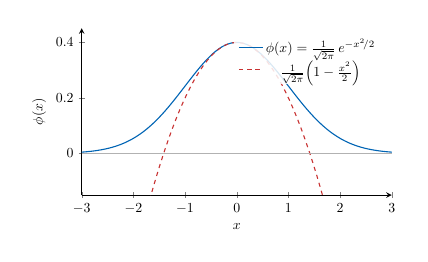
\begin{tikzpicture}[scale=0.5]
\begin{axis}[
    width=0.78\textwidth,
    height=0.48\textwidth,
    xlabel={$x$},
    ylabel={$\phi(x)$},
    xmin=-3, xmax=3,
    ymin=-0.15, ymax=0.45,
    axis lines=left,
    legend style={at={(0.97,0.97)}, anchor=north east, draw=none,
                  fill=white, fill opacity=0.85, text opacity=1},
    thick,
]
% Exact phi(x)
\addplot[accent, thick, smooth, domain=-3:3, samples=80]
    {1/sqrt(2*pi)*exp(-x^2/2)};
\addlegendentry{$\phi(x) = \frac{1}{\sqrt{2\pi}}\,e^{-x^2\!/2}$}
% Taylor approximation
\addplot[loss, thick, dashed, domain=-3:3, samples=80]
    {1/sqrt(2*pi)*(1-x^2/2)};
\addlegendentry{$\frac{1}{\sqrt{2\pi}}\!\left(1 - \frac{x^2}{2}\right)$}
% Zero line
\draw[black!30, thin] (axis cs:-3,0) -- (axis cs:3,0);
\end{axis}
\end{tikzpicture}
\caption{Standard normal PDF $\phi(x)$ and its second-order Taylor approximation.}
\label{fig:phi_approx}
\end{figure}

\begin{figure}[t]
\centering
\subfloat[Standard normal CDF $\Phi(x)$ and its first-order Taylor approximation]{
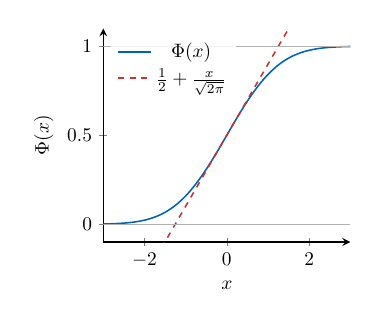
\begin{tikzpicture}[scale=0.7]
\begin{axis}[
    width=.5\textwidth,
    height=0.45\textwidth,
    xlabel={$x$},
    ylabel={$\Phi(x)$},
    xmin=-3, xmax=3,
    ymin=-0.1, ymax=1.1,
    axis lines=left,
    legend style={at={(0.03,0.97)}, anchor=north west, draw=none,
                  fill=white, fill opacity=0.85, text opacity=1},
    thick,
]
% Exact Phi(x) (tabulated from scipy)
\addplot[accent, thick, smooth, tension=0.6] coordinates {
    (-3.00,0.0013) (-2.90,0.0019) (-2.80,0.0026) (-2.70,0.0035)
    (-2.60,0.0047) (-2.50,0.0062) (-2.40,0.0082) (-2.30,0.0107)
    (-2.20,0.0139) (-2.10,0.0179) (-2.00,0.0228) (-1.90,0.0287)
    (-1.80,0.0359) (-1.70,0.0446) (-1.60,0.0548) (-1.50,0.0668)
    (-1.40,0.0808) (-1.30,0.0968) (-1.20,0.1151) (-1.10,0.1357)
    (-1.00,0.1587) (-0.90,0.1841) (-0.80,0.2119) (-0.70,0.2420)
    (-0.60,0.2743) (-0.50,0.3085) (-0.40,0.3446) (-0.30,0.3821)
    (-0.20,0.4207) (-0.10,0.4602) ( 0.00,0.5000) ( 0.10,0.5398)
    ( 0.20,0.5793) ( 0.30,0.6179) ( 0.40,0.6554) ( 0.50,0.6915)
    ( 0.60,0.7257) ( 0.70,0.7580) ( 0.80,0.7881) ( 0.90,0.8159)
    ( 1.00,0.8413) ( 1.10,0.8643) ( 1.20,0.8849) ( 1.30,0.9032)
    ( 1.40,0.9192) ( 1.50,0.9332) ( 1.60,0.9452) ( 1.70,0.9554)
    ( 1.80,0.9641) ( 1.90,0.9713) ( 2.00,0.9772) ( 2.10,0.9821)
    ( 2.20,0.9861) ( 2.30,0.9893) ( 2.40,0.9918) ( 2.50,0.9938)
    ( 2.60,0.9953) ( 2.70,0.9965) ( 2.80,0.9974) ( 2.90,0.9981)
    ( 3.00,0.9987)
};
\addlegendentry{$\Phi(x)$}
% Linear approximation
\addplot[loss, thick, dashed, domain=-3:3, samples=2]
    {0.5 + x/sqrt(2*pi)};
\addlegendentry{$\tfrac{1}{2} + \tfrac{x}{\sqrt{2\pi}}$}
% Reference lines
\draw[black!30, thin] (axis cs:-3,0) -- (axis cs:3,0);
\draw[black!30, thin] (axis cs:-3,1) -- (axis cs:3,1);
\end{axis}
\end{tikzpicture}\label{fig:Phi_approx}}
\qquad
\subfloat[Inverse normal CDF $\Phi^{-1}(\Delta)$ and its linear approximation.]{
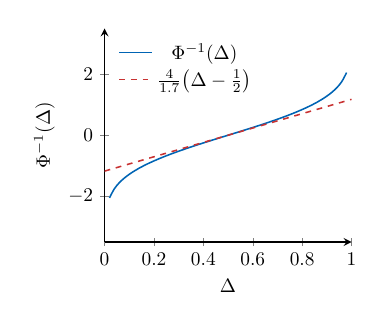
\begin{tikzpicture}[scale=0.7]
\begin{axis}[
    width=0.5\textwidth,
    height=0.45\textwidth,
    xlabel={$\Delta$},
    ylabel={$\Phi^{-1}(\Delta)$},
    xmin=0, xmax=1,
    ymin=-3.5, ymax=3.5,
    axis lines=left,
    legend style={at={(0.03,0.97)}, anchor=north west, draw=none,
                  fill=white, fill opacity=0.85, text opacity=1},
    thick,
]
% Exact (tabulated from scipy)
\addplot[accent, thick, smooth, tension=0.6] coordinates {
    (0.02,-2.054) (0.04,-1.751) (0.06,-1.555) (0.08,-1.405) (0.10,-1.282)
    (0.12,-1.175) (0.14,-1.080) (0.16,-0.994) (0.18,-0.915) (0.20,-0.842)
    (0.22,-0.772) (0.24,-0.706) (0.26,-0.643) (0.28,-0.583) (0.30,-0.524)
    (0.32,-0.468) (0.34,-0.412) (0.36,-0.358) (0.38,-0.305) (0.40,-0.253)
    (0.42,-0.202) (0.44,-0.151) (0.46,-0.100) (0.48,-0.050) (0.50, 0.000)
    (0.52, 0.050) (0.54, 0.100) (0.56, 0.151) (0.58, 0.202) (0.60, 0.253)
    (0.62, 0.305) (0.64, 0.358) (0.66, 0.412) (0.68, 0.468) (0.70, 0.524)
    (0.72, 0.583) (0.74, 0.643) (0.76, 0.706) (0.78, 0.772) (0.80, 0.842)
    (0.82, 0.915) (0.84, 0.994) (0.86, 1.080) (0.88, 1.175) (0.90, 1.282)
    (0.92, 1.405) (0.94, 1.555) (0.96, 1.751) (0.98, 2.054)
};
\addlegendentry{$\Phi^{-1}(\Delta)$}
% Linear approximation
\addplot[loss, thick, dashed, domain=0:1, samples=2] {4/1.7*(x-0.5)};
\addlegendentry{$\tfrac{4}{1.7}\!\left(\Delta - \tfrac{1}{2}\right)$}
\end{axis}
\end{tikzpicture}\label{fig:Phi_inv_approx}}
\label{fig:CDF_approximations}
\end{figure}


\section{Computational experiments}
\subsection{Estimation of model parameters}

Our model relies on the true distribution parameters $\mu, \Sigma$. However, as decision-makers we do not have access to them; we can only estimate from past data. Having access to stock data prices over a specified horizon, we split the horizon into $T$-many periods, with $t_k^+, t_k^-$ representing the `'opening`' and `'closing`' times of the period, respectively. WLOG, let us consider periods with lengths of at least 1 day. The opening time corresponds to the period's earliest possible trading time --- generally 9:30AM New York time on the first trading day of the period, while the closing time corresponds to the latest possible trading time --- generally 4PM New York time on the last trading day of the period. The `'opening price`' and `'closing price`' are the stock prices at the opening and closing times, respectively. 

Let $S_i(t)$ be the price of asset $i$ at time $t$. Note that $S_i(t_k^-) \not\equiv S_i(t_{k+1}^+)$ due to pre \& post-market trading. Define $r_i^k = \frac{S(t_k^-)-S(t_k^+)}{S(t_k^+)}$ to be the return of asset $i$ during period $k$. We thus estimate $\mu, \Sigma$ as
\begin{equation}\label{eq:estimation}
    \begin{aligned}
\mu_i &\approx \frac1T\sum_{k=1}^Tr_i^k  
\end{aligned}\qquad
\begin{aligned}
\Sigma_{ij} &\approx \frac{1}{T-1}\sum_{k=1}^T (r_i^k-\mu_i)(r_j^k-\mu_j)
\end{aligned}
\end{equation}
Since each stock's returns and variance can be significantly impacted by certain covariates --- i.e. economic and geopolitical conditions, we further refine each parameter by conditioning them on observable covariates. We assumed that each stock's return is normally distributed, thus let us define
\[
\mu = \begin{bmatrix}
    \mu_X \\
    \mu_Y
\end{bmatrix}, \Sigma = \begin{bmatrix}
    \Sigma_{XX} & \Sigma_{XY} \\
    \Sigma_{YX} & \Sigma_{YY}
\end{bmatrix}
\]
If $X \gauss(\mu_X, \Sigma_{XX})$ (the stock returns) and $Y \gauss (\mu_Y, \Sigma_{YY})$ (covariates), Gaussian conditioning tells us that $X \sep Y \gauss (\mu_{X|Y=a}, \Sigma_{X | Y =a})$, where the parameters become
\[
\begin{aligned}
    &\mu_{X | Y = a} = \mu_X +\Sigma_{XY} \Sigma_{YY}^{-1}(a-\mu_Y) \\
    &\Sigma_{X | Y = a} = \Sigma_{XX} - \Sigma_{XY}\Sigma_{YY}^{-1}\Sigma_{YX}
\end{aligned}
\]
, where $a \in \R^k$ is a vector of covariates. The mean and covariance of each covariate is estimated using the same method as for each asset, outlined in Eq.~\ref{eq:estimation}.
%We define $\mu(a) = \mu_{X|Y=a}$, and we define $\Sigma(a) = \Sigma_{X|Y=a}$.

\subsection{Computational parameters}

We used the \texttt{yfinance} and \texttt{pandas} Python packages to gather and analyze the stock-price data. The period used to estimate the model parameters was from January 1st 2000, to December 31st 2021, inclusive. This period was chosen for its wide range of economic conditions --- major recessions in 2001 \& 2008, wide ranging inflation conditions, and differing central bank regimes --- all the while being recent enough that our chosen assets have at least a decade of trading data. The period was segmented into quarters, with start dates of Jan 1st, Apr 1st, Jul 1st, and Oct 1st.

In the case of a stock having its initial public offering (IPO) in the middle of the training period, the first data point considered was its first full quarter of trading. For example, Alphabet (GOOGL) was first listed on the NASDAQ exchange on August 19th 2004. Thus, the first period considered was the quarter starting Oct 1st 2004, and ending Dec 31st 2004. In the case where two assets have a different number of trading quarters, their covariance was only estimated based on their shared trading history.

Covariates were chosen as inflation --- measured as the core Price Consumers Expenditures (PCE) index, and the Federal Reserve's Effective Fed Funds (EFF) rate. Both are critical in computing cashflows, and thus are widely used in the Discounted CashFlow (DCF) stock pricing model, which many analysts use to determine the fair market value of an asset.

Stocks were chosen as 11 top American companies, from widely different sectors and industries, as outlined in Table~\ref{table:companies}. We compared our portfolio against the S\&P 500 market index. 

\begin{table}[t]
    \centering
    \begin{tabular}{|c|p{3in}|}
\hline Company & Sector (Industry) \\ \hline
NVIDIA & Technology (Semiconductors) \\ \hline
Apple  & Technology (Consumer Electronics) \\ \hline
Alphabet (Google) & Communication Services (Internet Content \& Information) \\ \hline
Broadcom & Technology (Semiconductors) \\ \hline
Walmart  & Consumer Defensive (Discount Stores) \\ \hline
JPMorgan Chase & Financial Services (Banks) \\ \hline
Eli Lilly  & Healthcare (Drug Manufacturers) \\ \hline
Exxon Mobil & Energy (Oil \& Gas) \\ \hline
Coca-Cola & Consumer Defensive (Beverages) \\ \hline 
Lockheed-Martin & Industrials (Aerospace \& Defense) \\ \hline
Ford & Consumer Cyclical (Auto Manufacturers) \\ \hline
    \end{tabular}
    \caption{Chosen equities, with their sectors and industries}
    \label{table:companies}
\end{table}

Experiments were run on a desktop with an AMD Ryzen 5900X and 32GB of RAM, and run with stopping conditions of a 1 hour time-limit, or a duality gap of 1\%. We also restricted $\Delta \in [0.1, 0.9]$, guaranteeing that values of $\Delta_i$ stays within a range where the gap between the true functions and our approximations remains small. We chose our portfolio comparison periods to be 14 quarters, roughly representing the average length of time between market cycles \citep{bearmarkets}.

\section{Results}

Experiments were run with different combinations of economic conditions. The first set of conditions was at the start of 2022, the peak of the post-covid inflation. In response, the federal reserve had aggressively hiked interest rates, leading to a high inflation \& high interest rate environment, usually causes for a stock-market downturn. As illustrated in Table~\ref{table:stock_allocation}, the solution leads to a greatly diversified portfolio, with put options far OTM. This could be due to the increase in price of options in high RFR, which pushes the price of options higher. Additionally, puts are collateralized with cash, thus high inflation leads to further increases in put prices, due to the time-value of the money being tied up in collateral. Thus our model prefers the free variance reduction of diversification over high insurance rates. We do note that even far ITM can have a significant impact on smoothing out large downward moves. For example on Liberation Day --- April 2nd 2025, the day large sweeping tariffs were announced --- the peak to trough return was -9.6\% for our put-protected portfolio (PPP), while it was -13.1\% for the unprotected portfolio, and -11.8\% for the market index. This shows a significant improvement in fast and large downside moves, which are typical of market crashes, as the saying goes `'the market takes the stairs up, and the elevator down.`' This is further reflected in Table~\ref{tab:result_metrics}, where the PPP enjoys larger returns and smaller variance then the unprotected portfolio, leading to a 12.8\% improvement in Sharpe Ratio. Both portfolio significantly outperform the benchmark, with only a 27.3\% and 41.3\% increase in variance, respectively, resulting in almost a quadrupling of the Sharpe Ratio for the PPP over the benchmark (Fig.~\ref{fig:portfolio_graph}).

\begin{table}[!h]
    \centering
    \subfloat[Solution stock \& put allocation]{\begin{tabular}{|c|c|c|}
\hline Ticker & Weight & Delta \\ \hline
NVDA &  8.84\% & 0.1 \\ \hline
AAPL &  5.2\% & 0.1 \\ \hline
AVGO &  27.05\% & 0.1 \\ \hline
LLY &  9.25\% & 0.1 \\ \hline
XOM &  21.02\% & 0.1 \\ \hline
KO &  7.48\% & 0.1 \\ \hline
LMT &  21.15\% & 0.1 \\ \hline
    \end{tabular}
    \label{table:stock_allocation}}
    \qquad\qquad
    \subfloat[Solution result metrics]{
    \begin{tabular}{|c|c|c|c|}
        \hline Asset & $\mu$ & $\sigma$ & SR \\ \hline
        Portfolio & 0.0791 & 0.1101 & 0.618 \\ \hline 
        Put port. & 0.0802 & 0.0992 & 0.6969 \\ \hline 
        Benchmark & 0.0249 & 0.0779 & 0.1774 \\ \hline 
           \end{tabular}
           \label{tab:result_metrics}
    }
    \caption{Portfolio structure and performance metrics}
\end{table}

\begin{figure}[!h]
    \centering
    \subfloat[Portfolio performance]{
    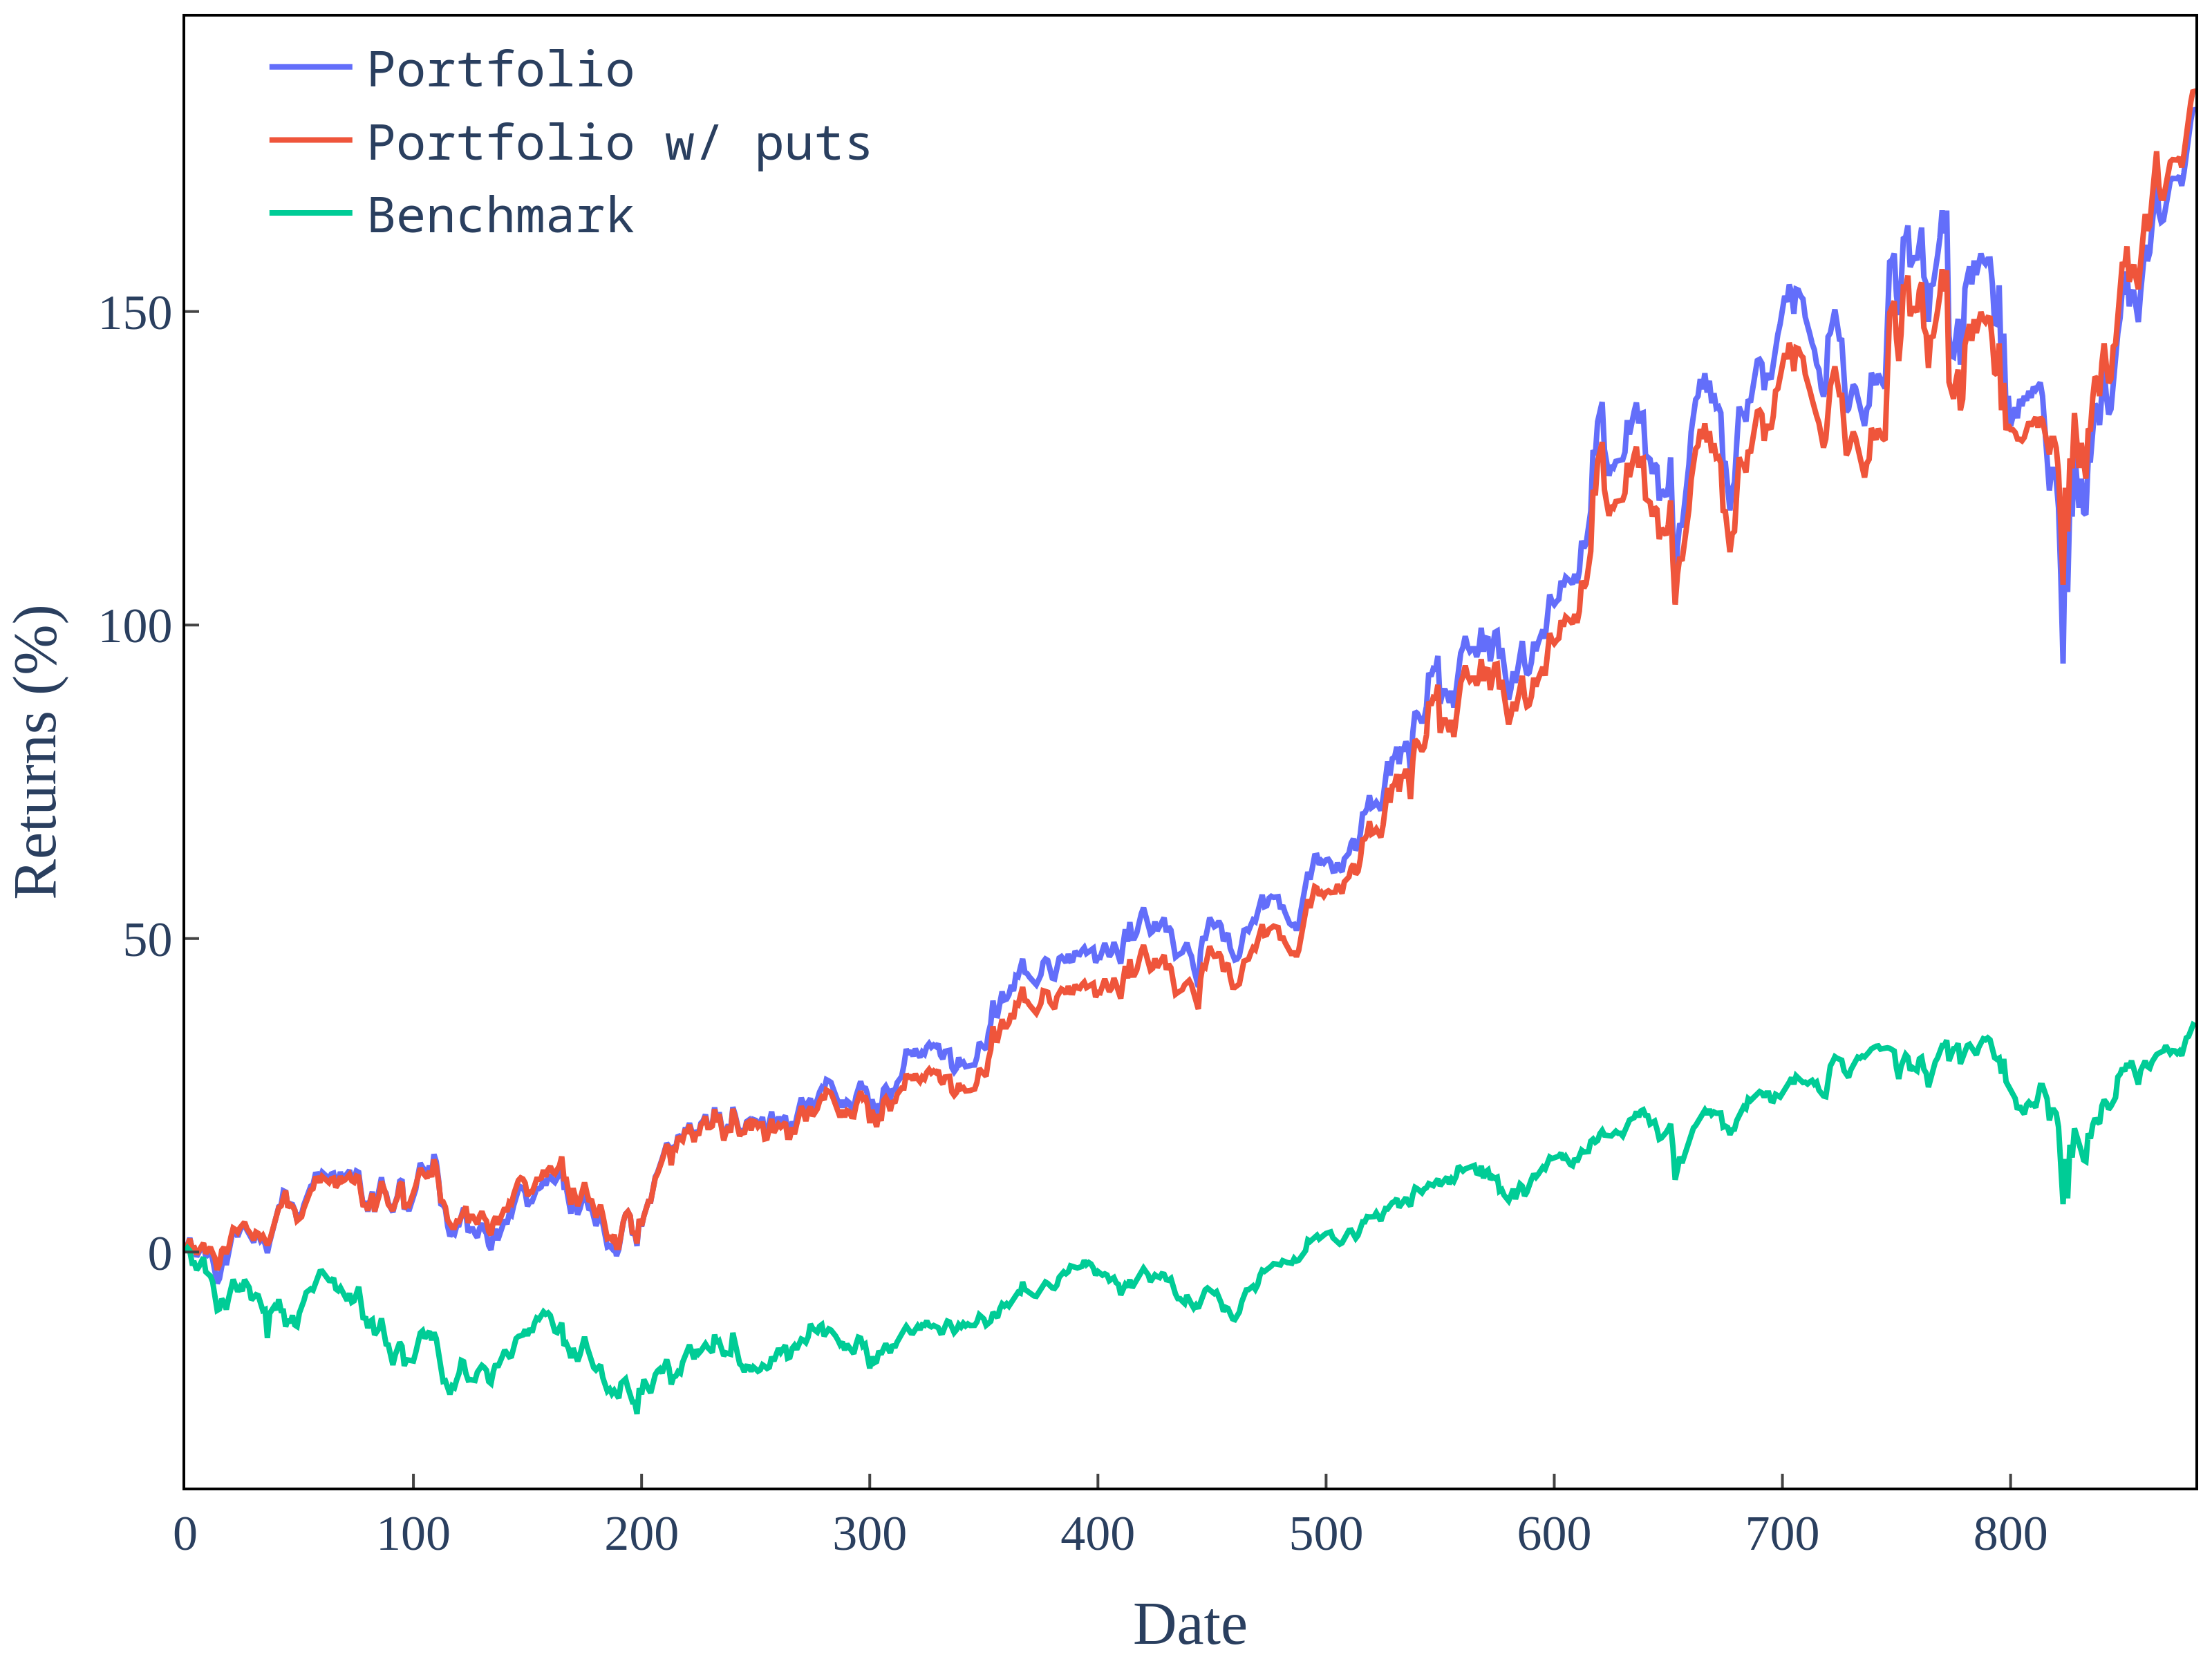
\includegraphics[width=0.5\linewidth]{graphs/(0.022, 4.5)_max_sharpe_20260506192031.png}
    \label{fig:portfolio_graph}
    }
    \subfloat[Duality gap over time]{
    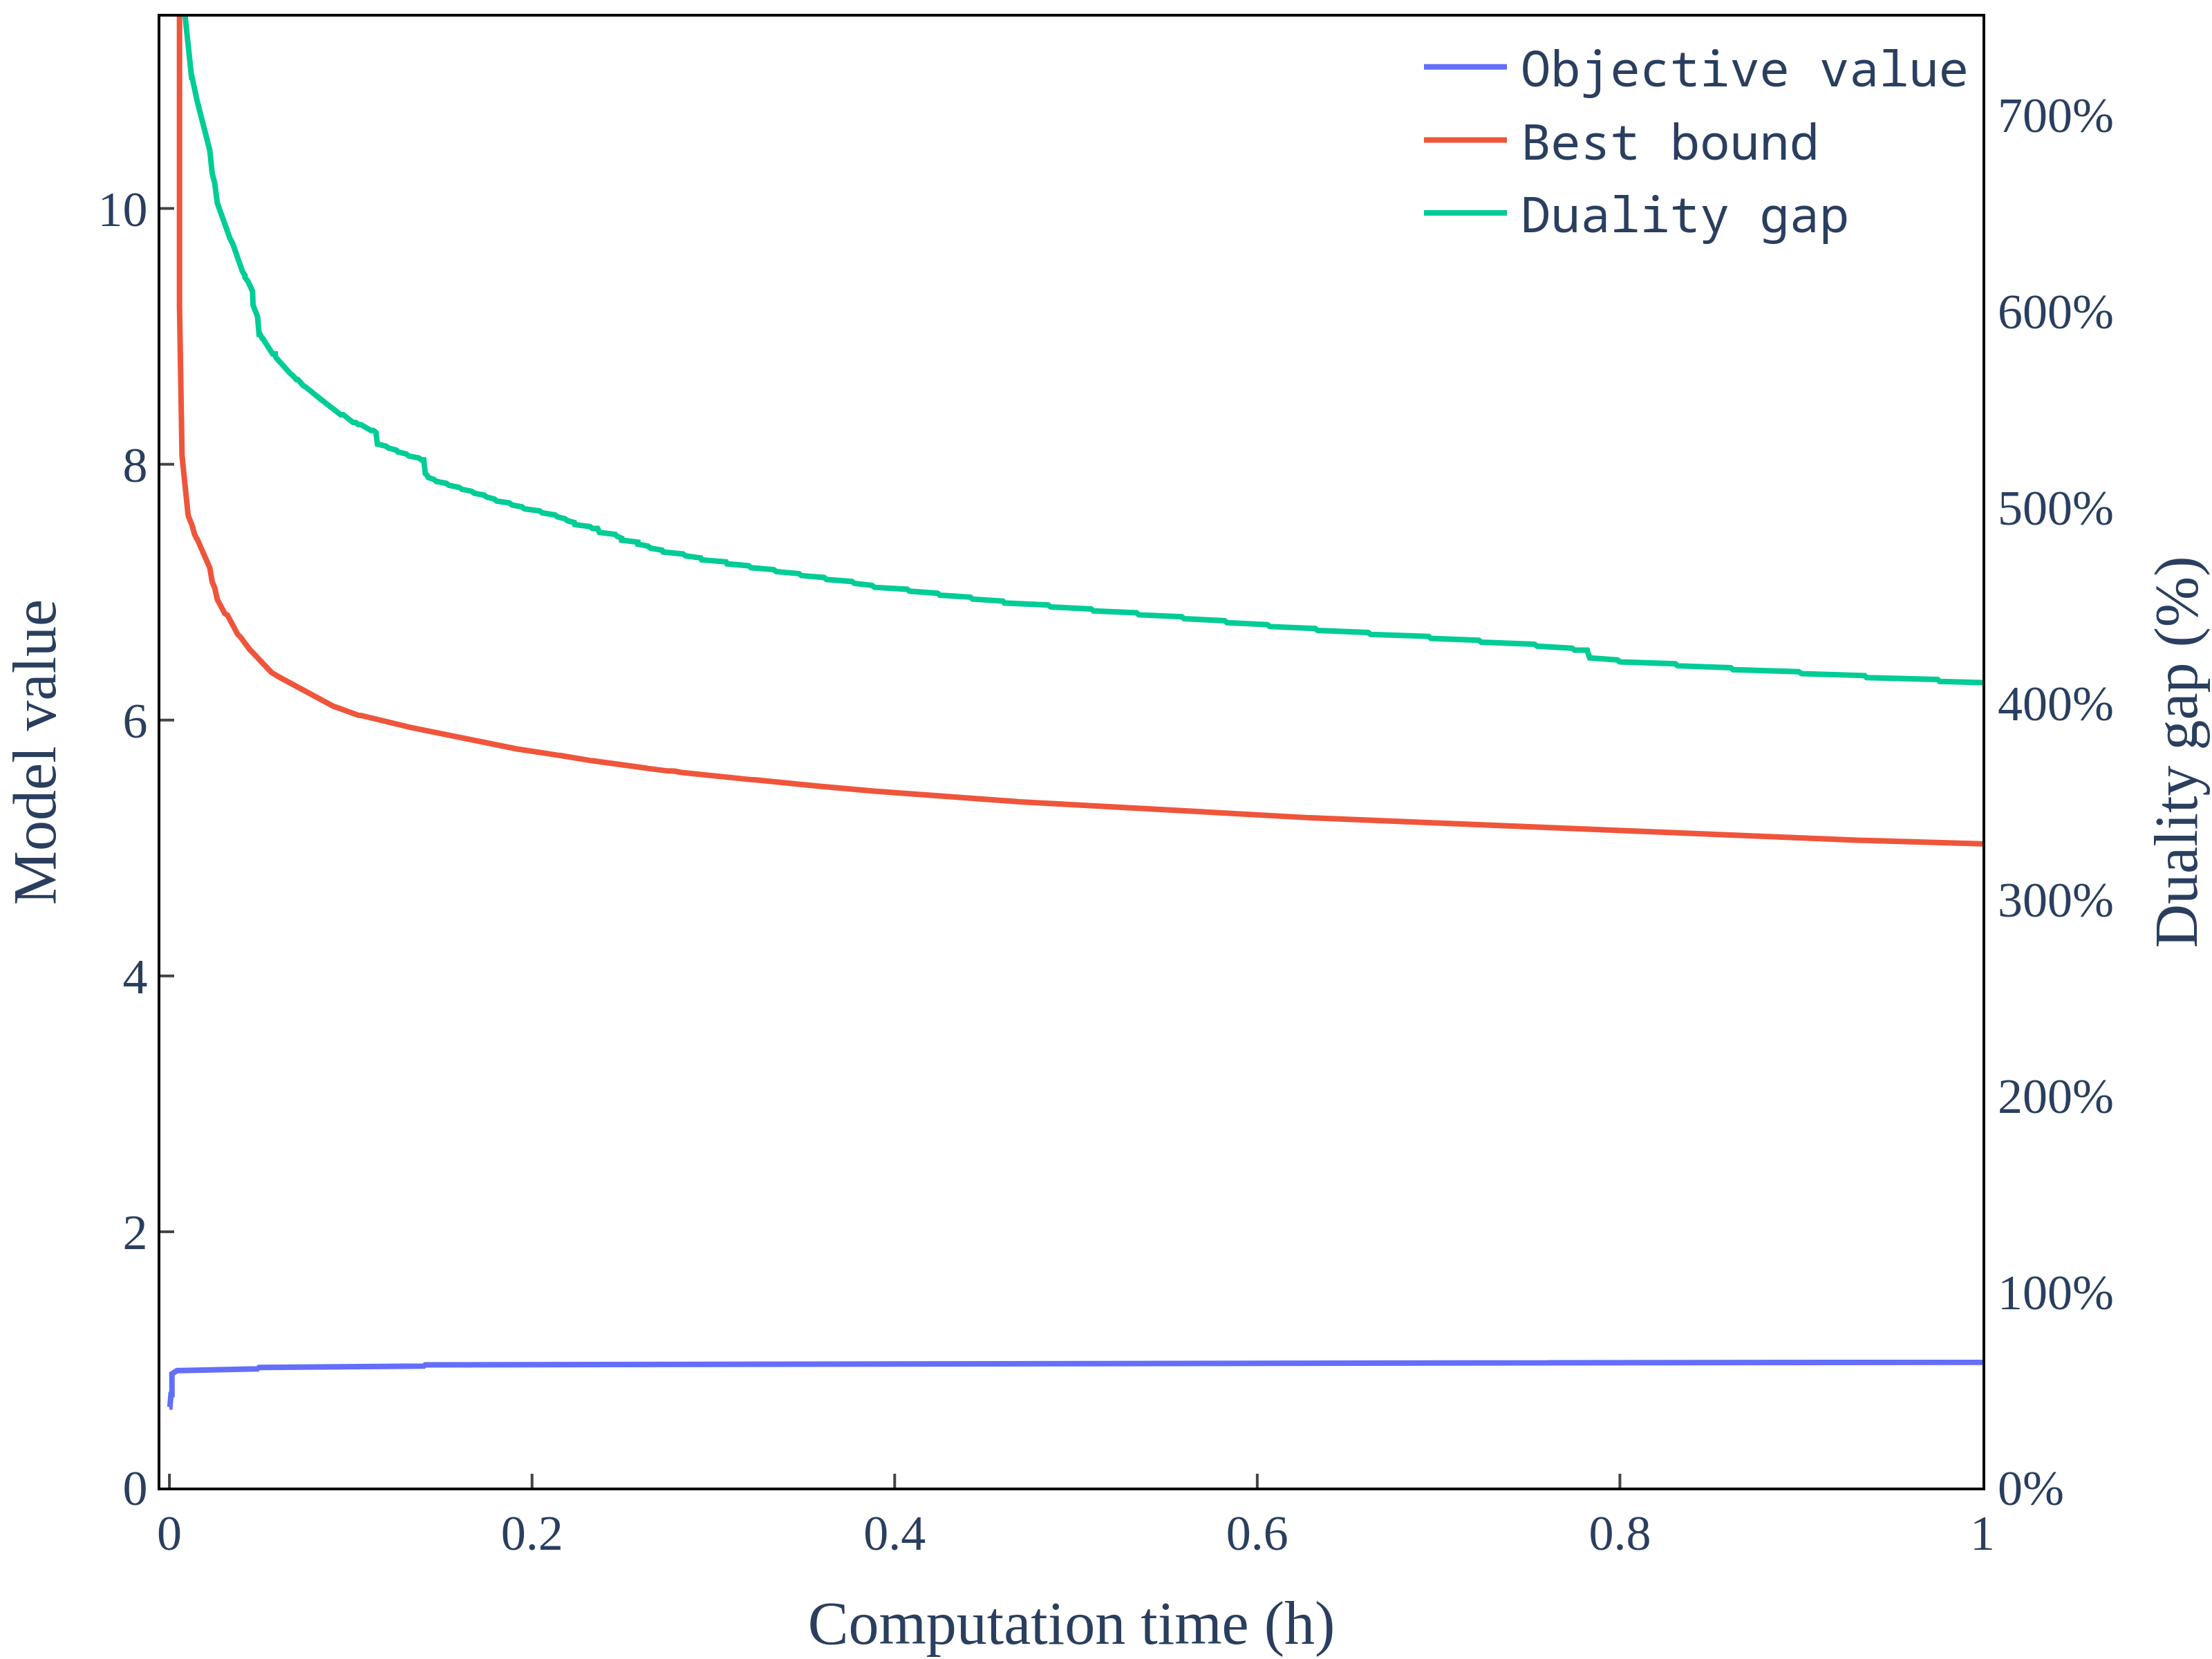
\includegraphics[width=0.5\linewidth]{graphs/duality_gap_9_4.5.png}
    \label{fig:duality_gap}
    }
    \caption{Daily portfolio performance and computational evolution}
\end{figure}

\section{Conclusion}

As observed, in certain market conditions, put options can offer a reduction in the variance of a portfolio, at minimal to no-cost in terms of returns. However, due to the highly non-linear nature of options and censored normal distributions, approximations must be made to solve the problem efficiently. Even with those, the duality gap remains large after an hour of computation (Fig.~\ref{fig:duality_gap}). Future advances should include a tailored solution method. With the true problem (Eq~\ref{eq:objective}) being CQr for fixed $\Delta$, it might be particularly amiable to decomposition methods, or Block Coordinate Descent algorithms.

\newpage
\bibliography{Paper}

\section{Appendix}

\textbf{AI Usage:} We used Claude while drawing Figures \ref{fig:protective_put}, \ref{fig:phi_approx}, \ref{fig:Phi_approx}, \ref{fig:Phi_inv_approx}. We also used Claude to troubleshoot some bugs when generating graphs with Plotly in Python.

\subsection{Results for conditions at the start of 2023 (3\% inflation, 5\% RFR)}

Further analysis into high-return market regimes shows that our approach yields significantly higher returns above the market, but that the addition of options can reduce the Sharpe ratio. Therefore, decision-makers should carefully evaluate the macro-economic environment to determine whether downside protection is needed at all.

\begin{table}[!h]
    \centering
    \subfloat[]{
    \begin{tabular}{|c|c|c|}
\hline Ticker & Weight & Delta \\ \hline
NVDA &  12.36\% & 0.14 \\ \hline
AAPL &  2.37\% & 0.47 \\ \hline
GOOG &  25.97\% & 0.3 \\ \hline
AVGO &  6.67\% & 0.24 \\ \hline
LMT &  52.63\% & 0.15 \\ \hline

    \end{tabular}

}
\subfloat[]{

    \begin{tabular}{|c|c|c|c|}
\hline Asset & $\mu$ & $\sigma$ & SR \\ \hline
Portfolio & 0.1038 & 0.1349 & 0.6785 \\ \hline 
Put port. & 0.0944 & 0.1311 & 0.6263 \\ \hline 
Benchmark & 0.0445 & 0.0597 & 0.5408 \\ \hline 
   \end{tabular}
}
\end{table}
\begin{figure}[!h]
    \centering
    \subfloat[Portfolio performance]{
    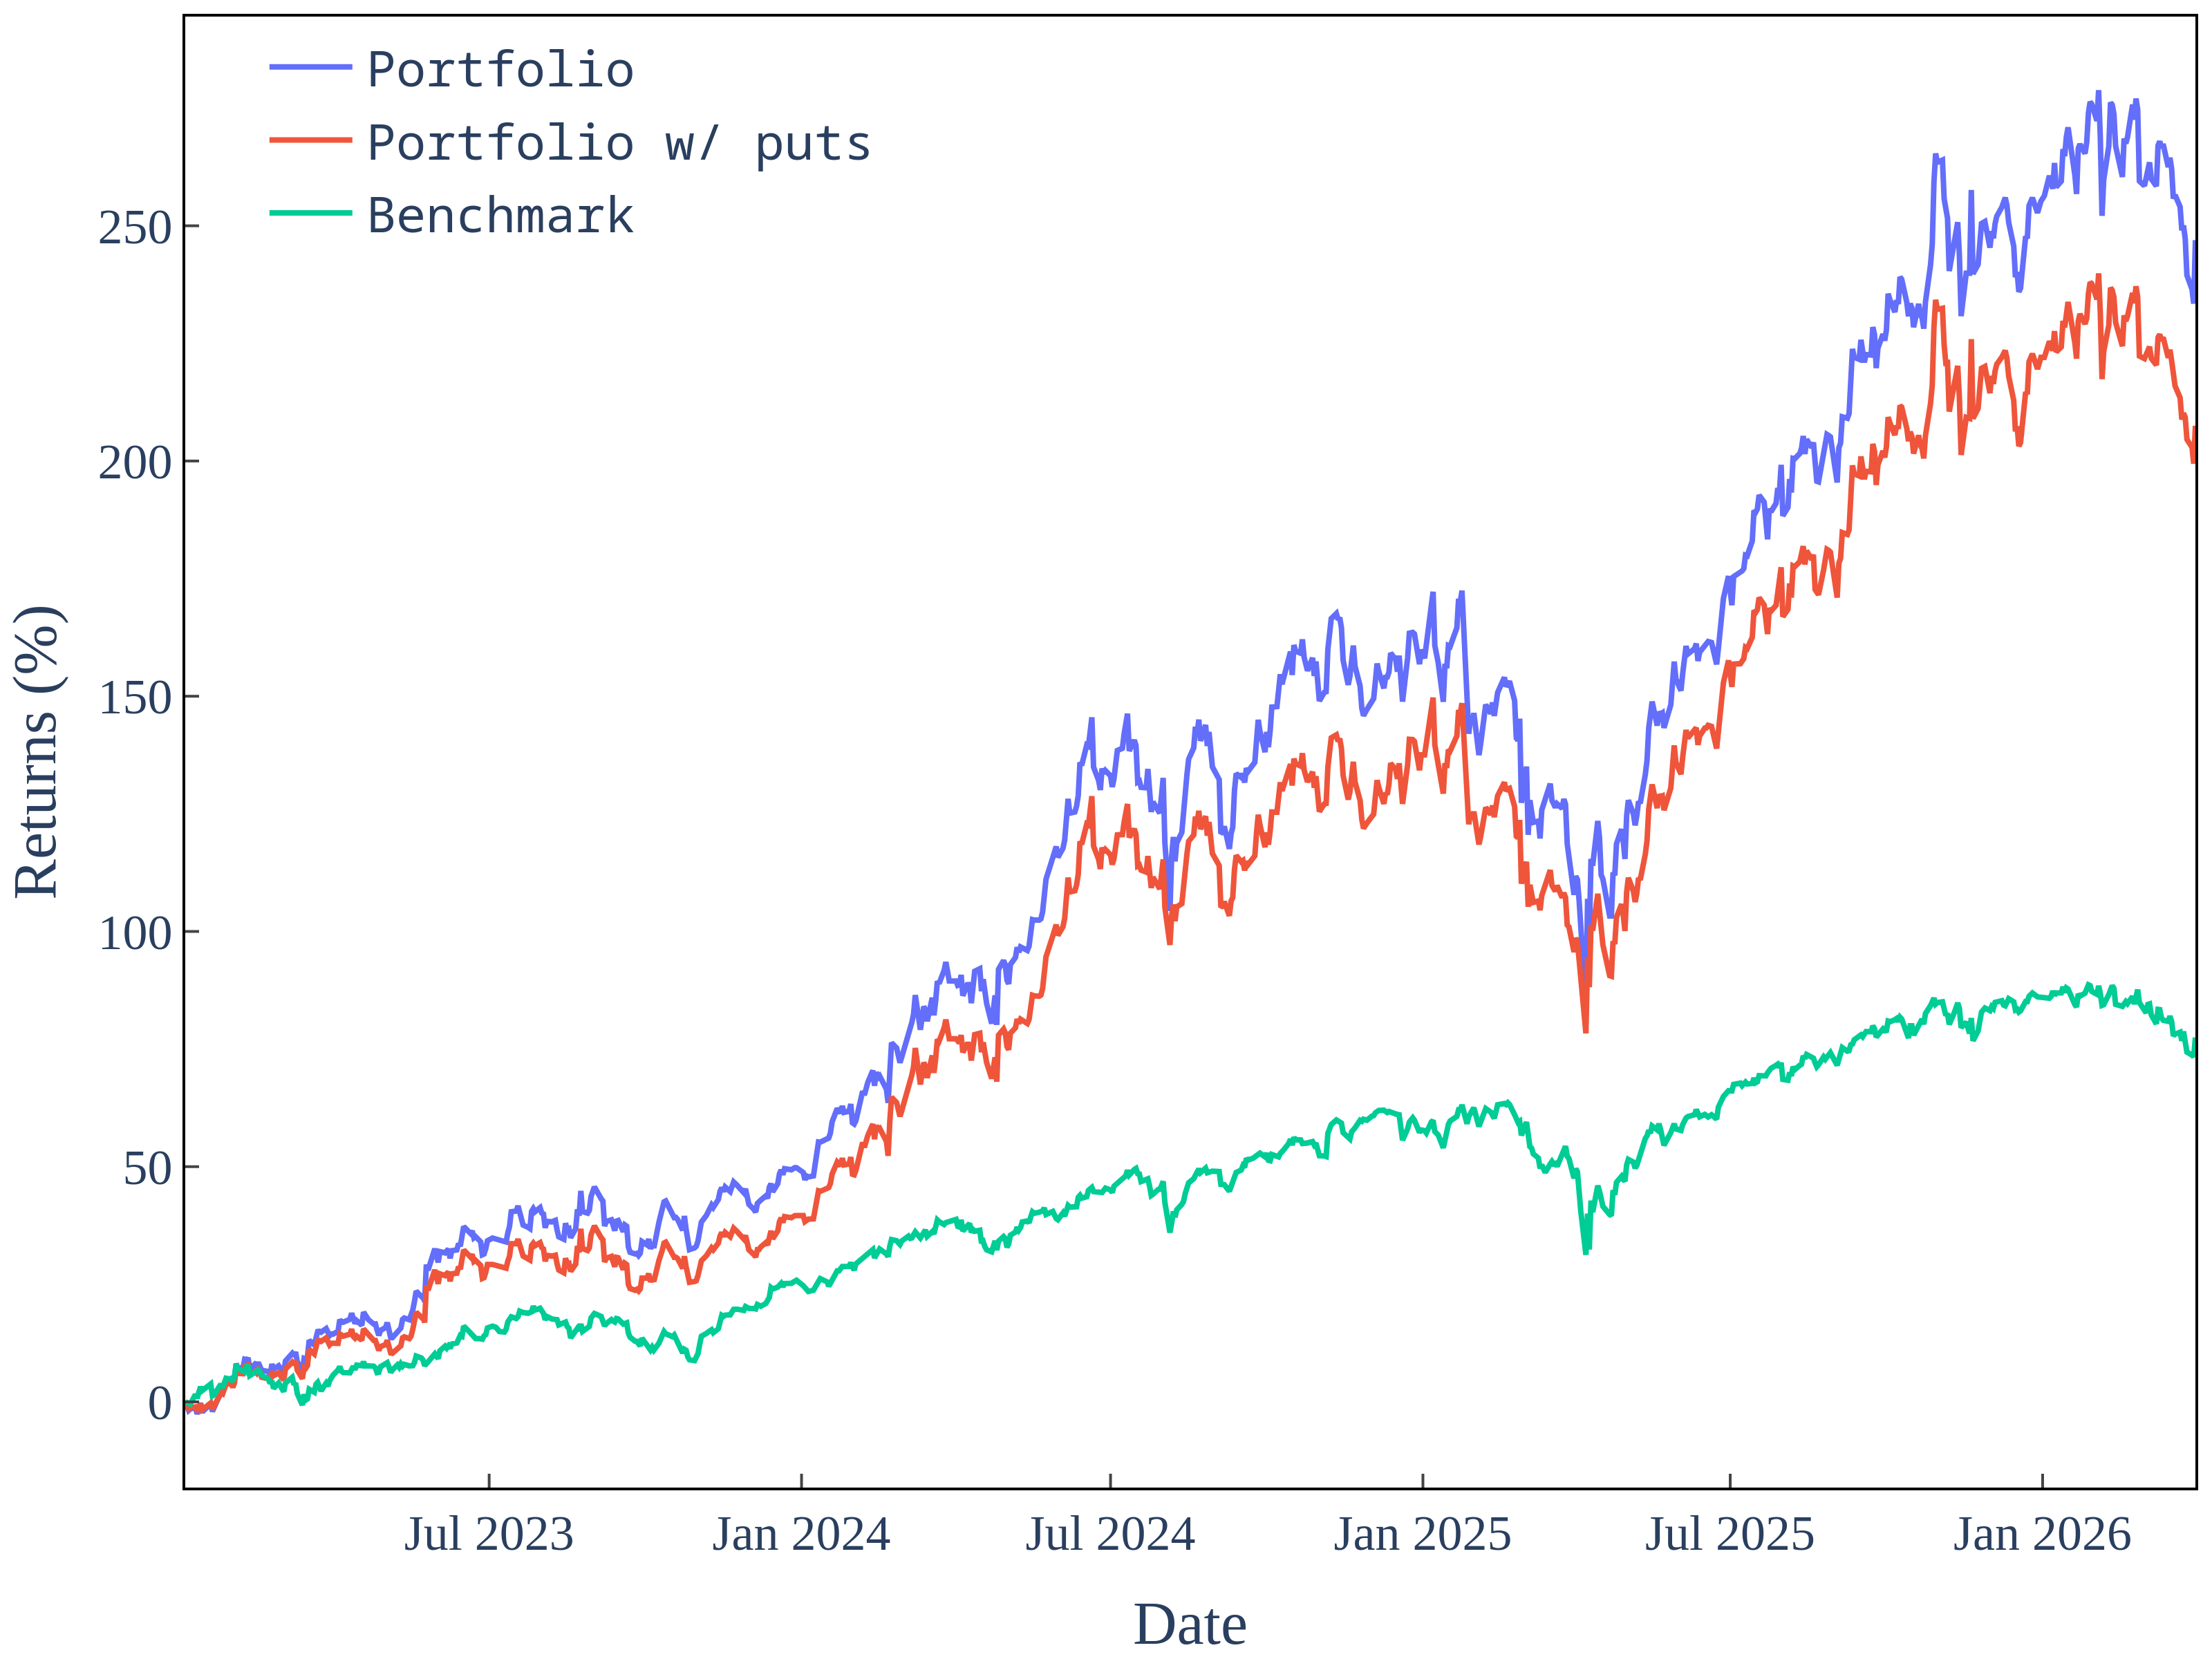
\includegraphics[width=0.5\linewidth]{graphs/(0.00742, 5)_max_sharpe_20260507114839.png}
    \label{fig:portfolio_graph_extra}
    }
    \subfloat[Duality gap over time]{
    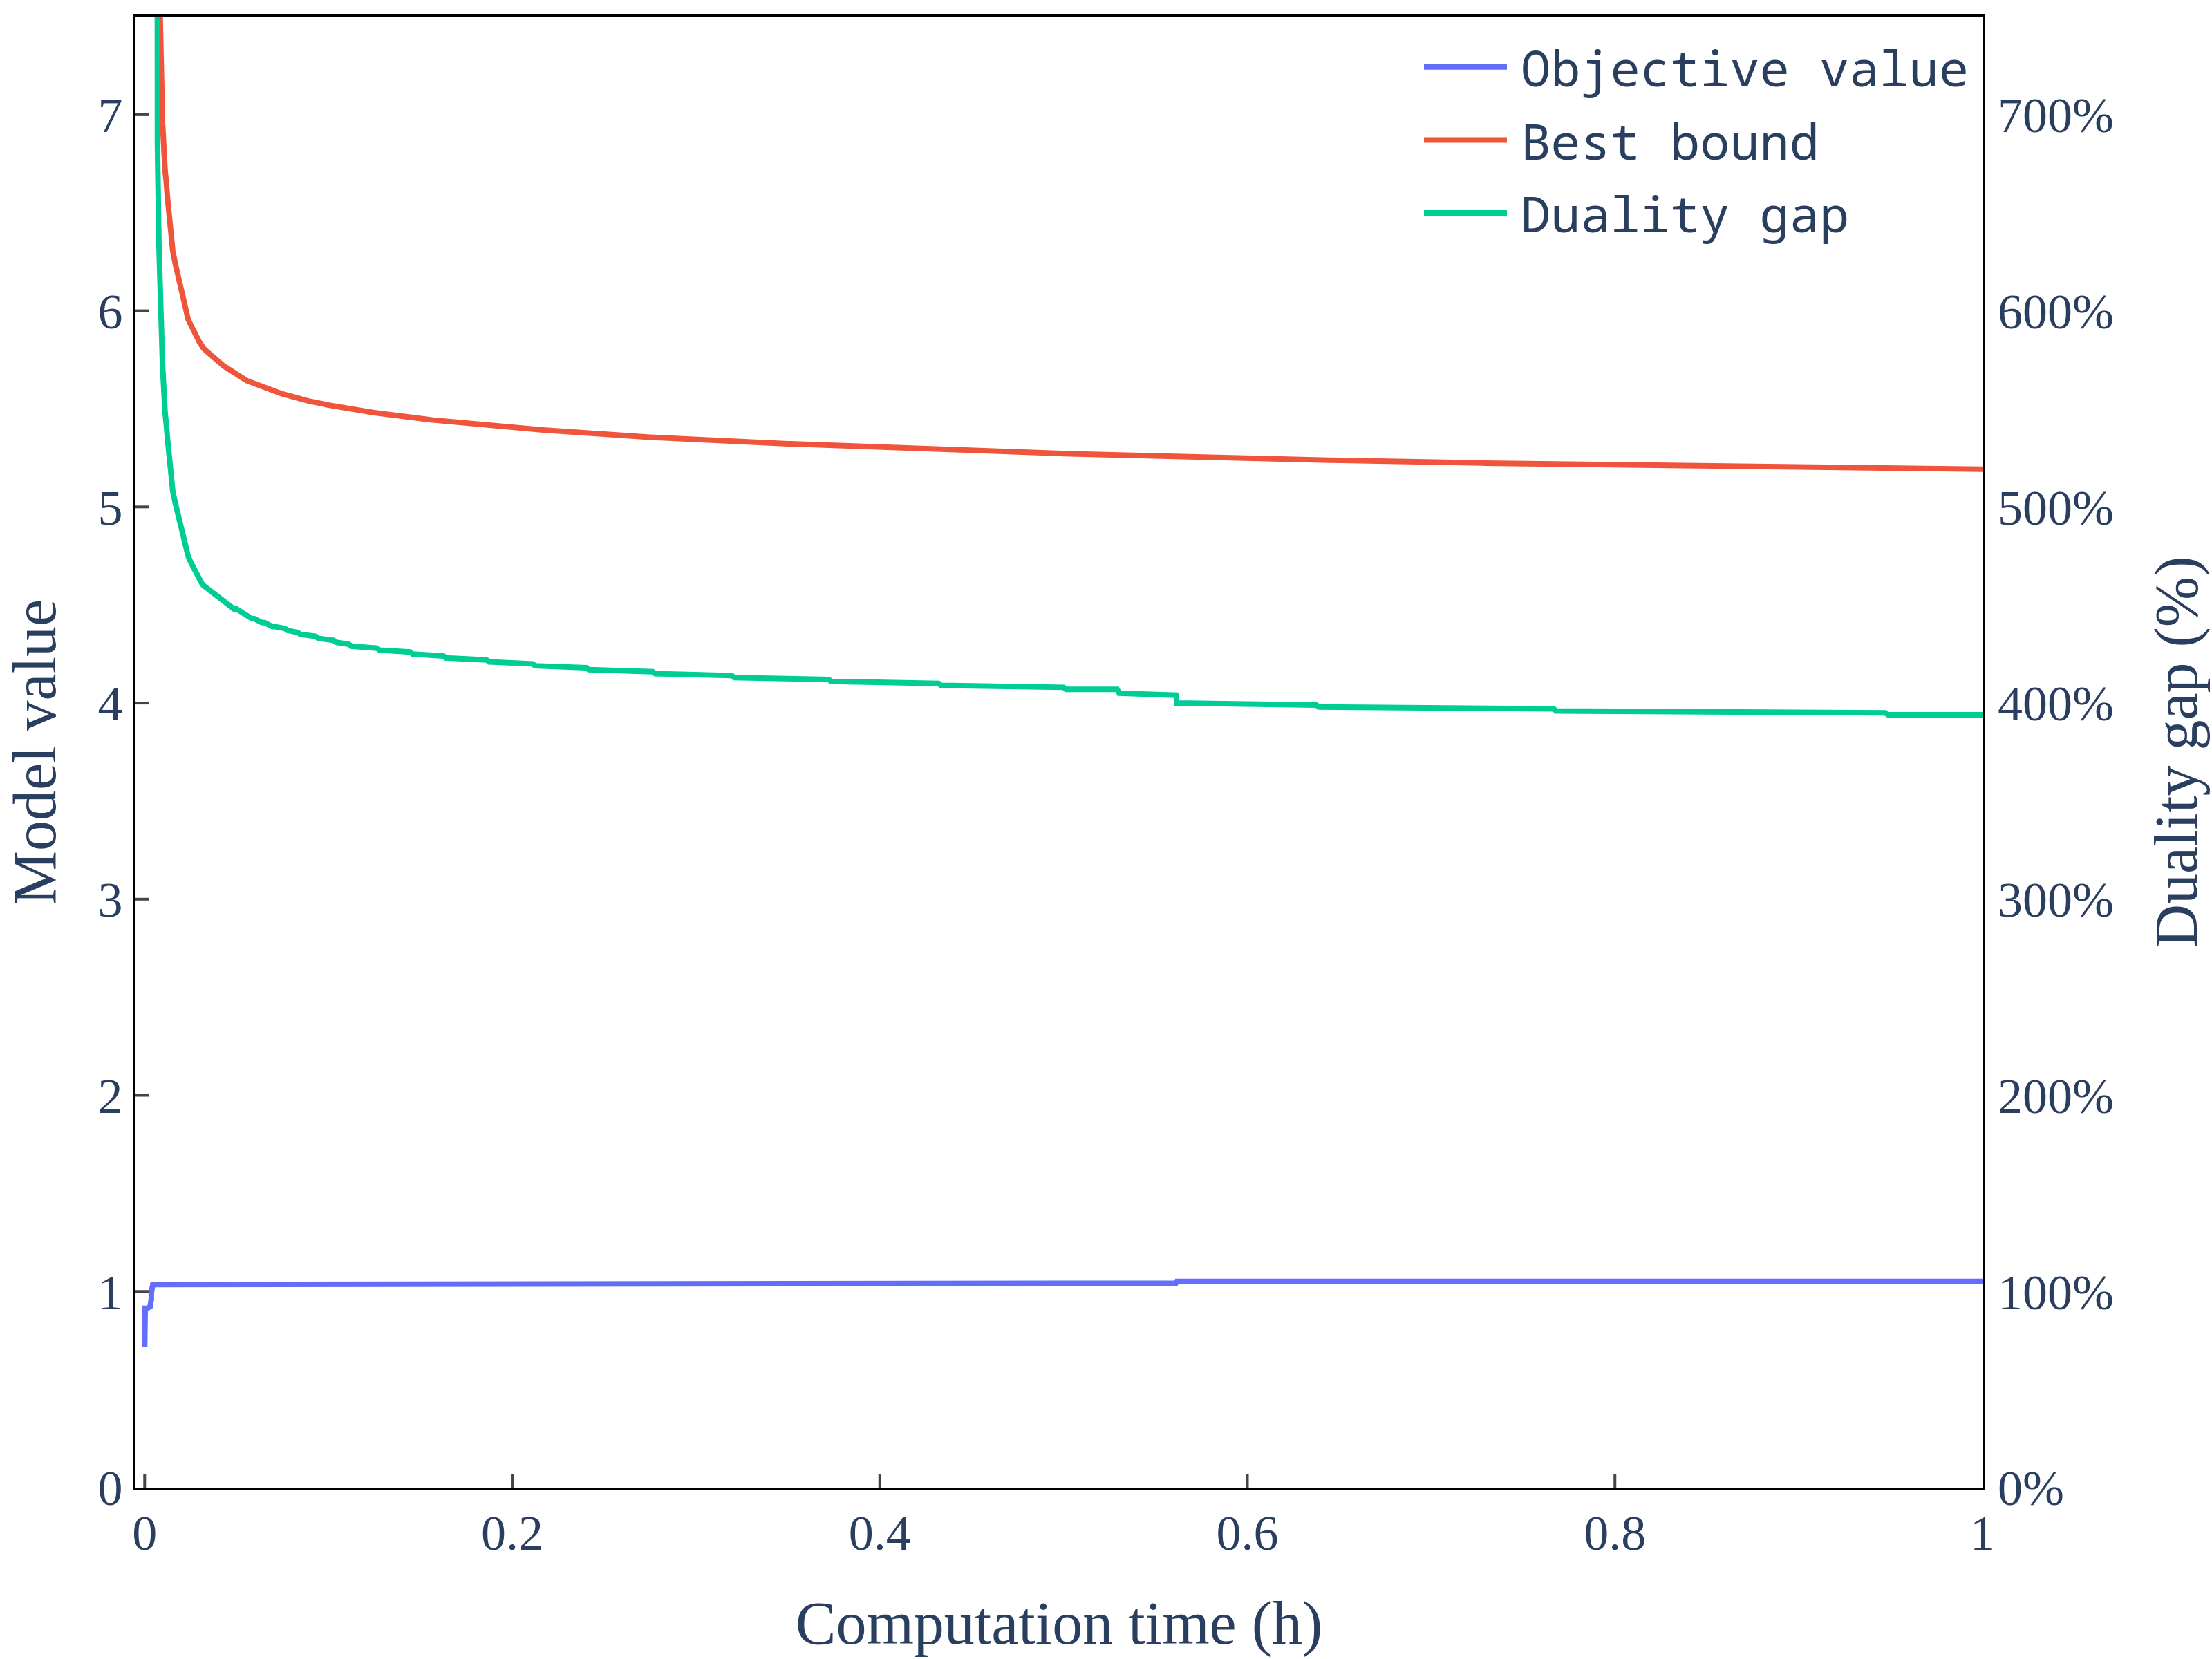
\includegraphics[width=0.5\linewidth]{graphs/duality_gap_2_3.png}
    \label{fig:duality_gap_extra}
    }
\end{figure}
\begin{figure}[!h]
    \centering
    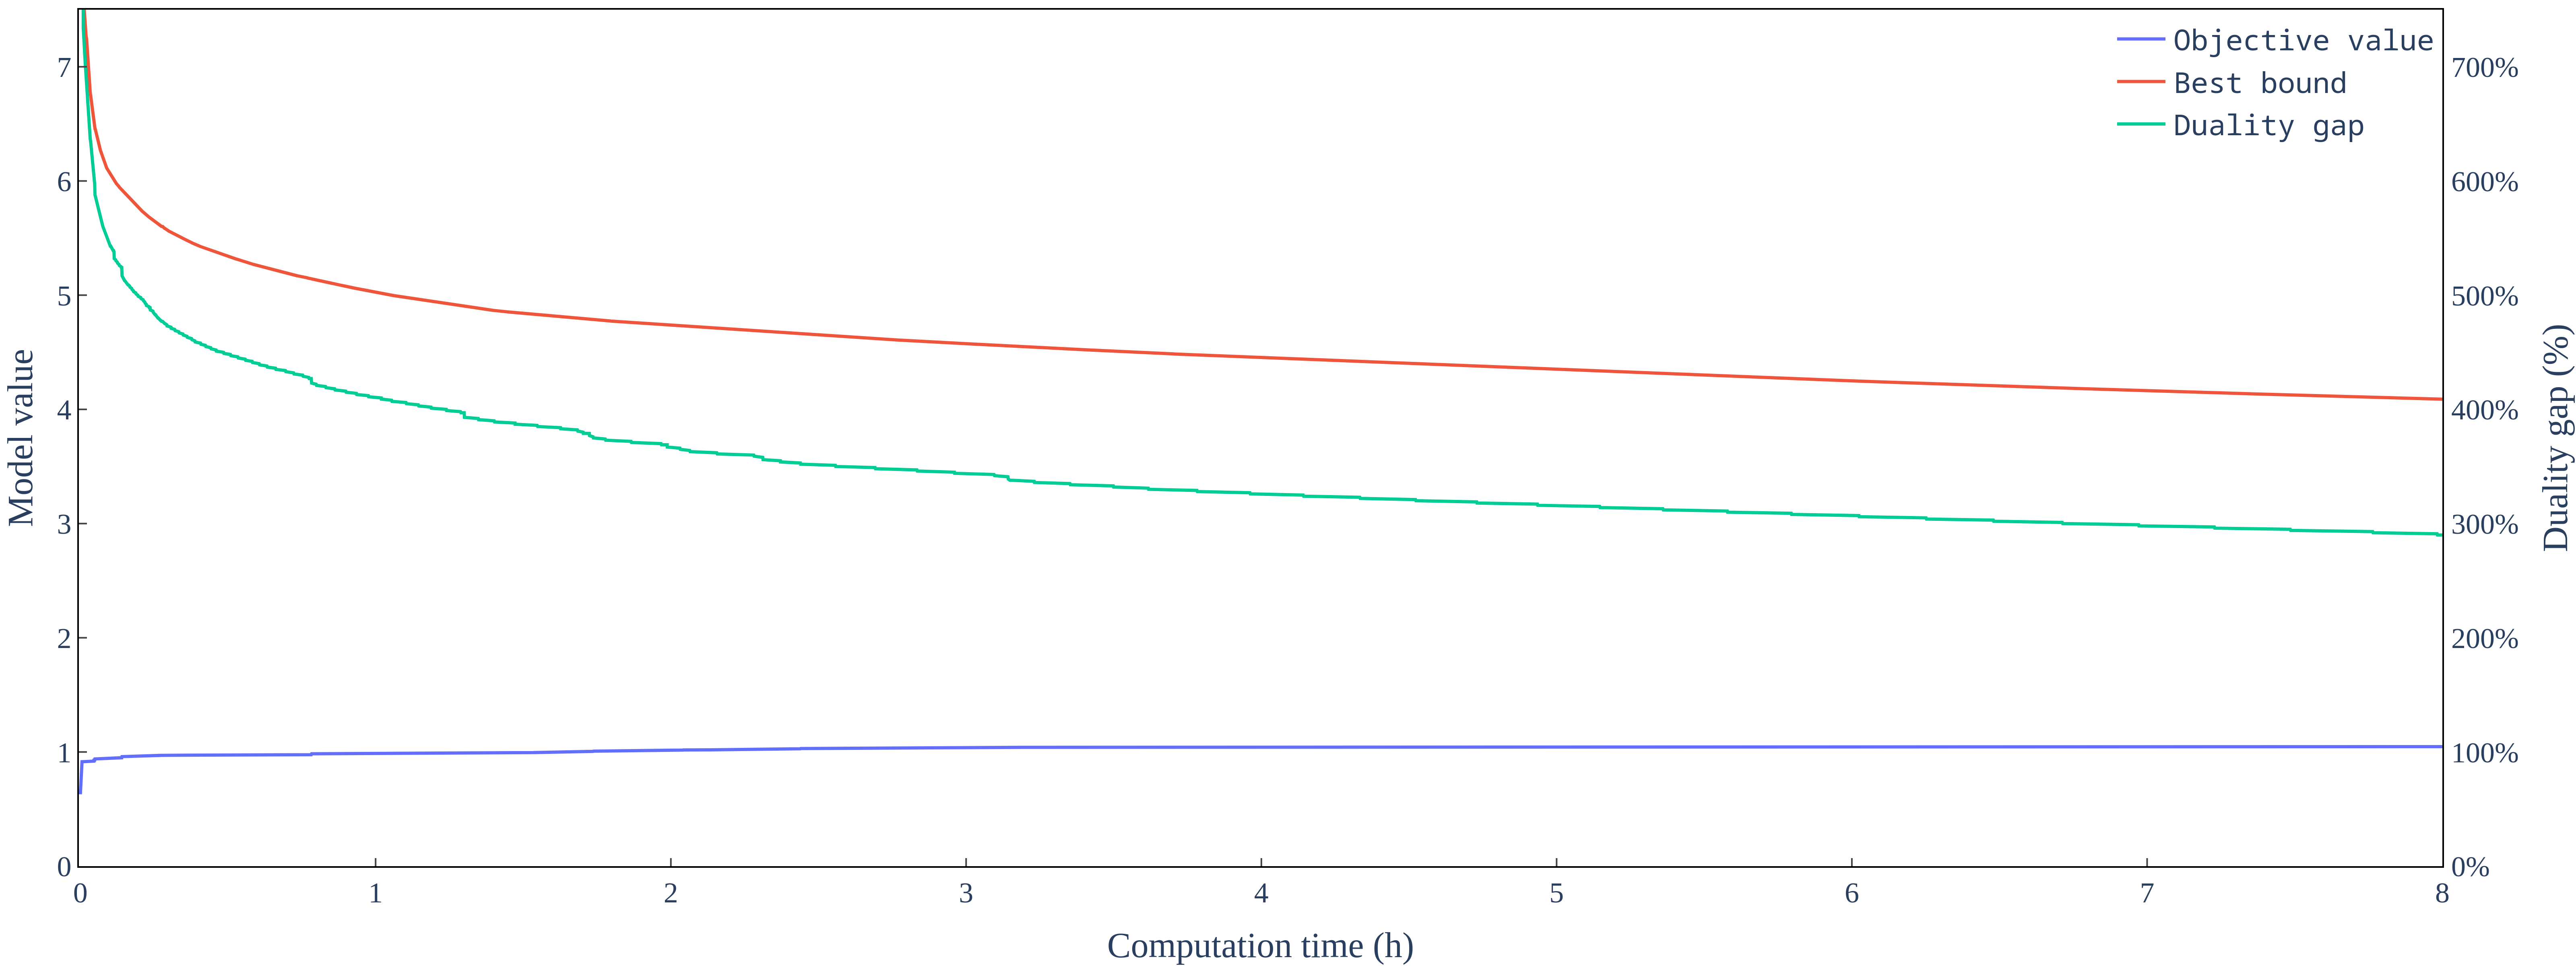
\includegraphics[width=1\linewidth]{graphs/duality_gap_3_5_xl.png}
    \label{fig:duality_gap_extra}
    \caption{Duality gap over time, over 8 hours}
\end{figure}

\end{document}
